\documentclass{article}

	\usepackage[margin=1in]{geometry}
	
	\usepackage[backend=bibtex, style=authoryear]{biblatex}
		
	\addbibresource{sources/sources.bib}
	\usepackage{hyperref}
	
			\title{\textsc{Neural Networks for Computed Tomography Imaging Spectrographs}}
			\date{\today}
			\author{Roy Smart \\ \url{roy.smart@montana.edu} \\ Montana State University, Department of Physics \\ Bozeman, MT 59717, USA}
			
	\usepackage{float}
	\usepackage{graphicx}
	\usepackage{subcaption}


\begin{document}

	\maketitle
	
	\tableofcontents
	
	\begin{abstract}
		
	\end{abstract}
		
	
	\section{Problem Statement}
		\subsection{Background}
		
			The solar atmosphere is an immense structure with a spectrum composed of numerous emission lines ranging from UV to X-rays. Properties of these emission lines such as intensity, wavelength and linewidth allow us to derive velocities, densities, and temperatures of the plasma composing the solar atmosphere. Measurements of these quantities at high spatial, spectral, and temporal resolution is essential to understanding the solar atmosphere and to satisfying the Heliophysics Division's goal of acquiring the ability to predict space weather events. Instruments known as spectrographs are used to measure the spectrum of the Sun with a spectral resolution large enough to characterize individual emission lines.
					
			Conventional spectrographs such as the Interface Region Imaging Spectrograph \textit{IRIS} (\cite{De Pontieu2014}), use a slit to restrict the spatial field of view along one direction and then uses a diffractive optical system to form images of the slit in one outboard order. This configuration yields images that represent the intensity of the light source as a 2D function of space (perpendicular to the dispersion direction) and wavelength. To acquire intensity information along the dispersion direction, conventional spectrographs are often operated in raster mode, where the slit is scanned parallel to the dispersion direction. This process builds up a \textit{spatial-spectral cube} (SSC), which contains the intensity of the light source as a 3D function of space (across a 2D field of view) and wavelength. Unfortunately the SSC acquired through the process of rastering is not cotemporal, i.e. each of the images within the SSC was taken at a different time, governed by the readout speed of the imager and the scanning speed of the slit. 		
		
			A c\textit{computed tomography imaging spectrograph} (CTIS) is a relatively new type of instrument design that shows promise in recovering a cotemporal SSC. These instruments have been independently developed for various scientific fields by multiple parties including: \cite{Okamoto:91}, \cite{bulygin:92}, \cite{Descour:95}, and \cite{kankel1}. A CTIS is able to measure a cotemporal SSC by eliminating the slit employed by the conventional slit spectrograph, and thus allows light from a wide field of view in both spatial directions to be imaged by the instrument. This modification would create an unresolvable ambiguity on images produced by a conventional spectrograph since it would be impossible to determine whether a unit of intensity at a particular location on an image originated from that location or was dispersed from an adjacent location. A CTIS attempts to resolve this ambiguity by forming images at multiple diffraction orders which provides enough information for computational techniques to reconstruct the SSC (\cite{inversion})
				
			 
		\subsection{Inversion}
			\label{inv_sec}
		
			Computing the spatial spectral cube using images formed at multiple diffraction orders can be interpreted as a classic 3D tomography problem where $N$ projections are taken through a translucent 3D object in $x$, $y$ and $\lambda$ space (\cite{Bulygin:05}).
			\begin{figure}[h!]
				\centering
				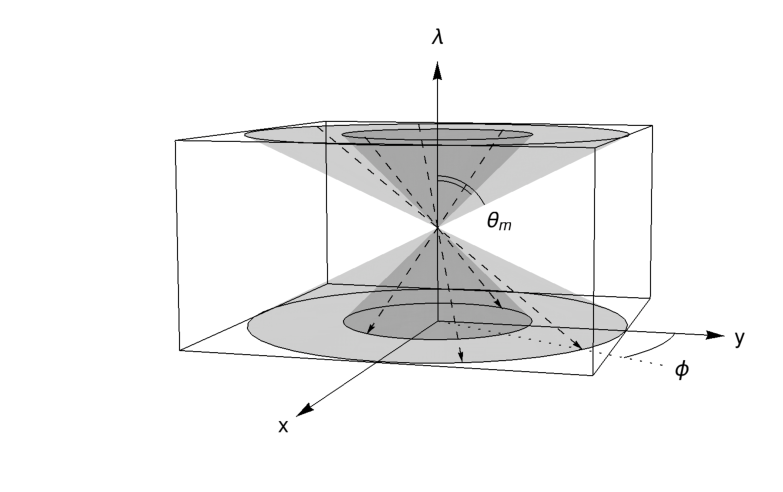
\includegraphics[width=0.75\textwidth]{figures/tomography}
				\caption{Geometry of the inversion problem for CTIS interpreted as a 3D tomography problem. $\theta_m$ describes the angle of the tomographic projection at each diffraction order and takes on discrete values, visualized by the nested cones. $\phi$ describes the dispersion direction and accepts continuous values. The four dotted lines are examples of particular projections through the spatial-spectal cube. Figure adapted from \cite{Bulygin:05}}
				\label{tomography}
			\end{figure}
			
			Using this representation, we can write the intensity in each order, $I_m$, of an object $v(x,y,\lambda)$ viewed by a CTIS in terms of the intergral equation provided by \cite{fox1}
			\begin{equation}
				I_m (x',y') = \int_B v(x' - \lambda \tan \theta_m \cos \phi, \; y' - \lambda \tan \theta_m \sin \phi, \; \lambda) \; d\lambda,
				\label{tomo_eqn}
			\end{equation}
			where $x'$ and $y'$ are image coordinates and $B$ is the passband of the instrument. Equation \ref{tomo_eqn} is a Fredholm integral equation of the first kind (\cite{RHB}) with a projection kernel. Our goal is then to invert Equation \ref{tomo_eqn} to recover the object $v(x,y,\lambda)$.
			
			The CTISs developed by Charles Kankelborg and his research group only take between $N=3$ and $N=6$ projections through the spatial-spectral cube. This limited number of projections does not provide enough information to completely reconstruct the spatial-spectral cube, i.e. in the case of the CTISs discussed below (MOSES and ESIS), inverting Equation \ref{tomo_eqn} is an ill-posed problem (\cite{inversion}). We can see this by noting that for a spatial spectral cube of length $L$ in both spatial directions, and a depth $M$ in the spectral direction the amount of information in the cube is $I_c = L^2 \times M$ and the the information provided by all the projections is $I_p = L^2 \times N$. Therefore, an inversion algorithm must to use physical constraints to have enough information to reconstruct the spatial-spectral cube (\cite{inversion}). In Section \ref{pwork} we will briefly explore advantages and disadvantages of the physical constraints used by current inversion algorithms, and in Section \ref{prop_sol} we will propose to use machine learning algorithms to approximate these physical constraints and solve the inversion problem.
			
		\subsection{Current and Planned CTISs}

			In the sections below, we will conduct a limited overview of the current and planned CTISs designed and built by Charles Kankelborg and his research group. A brief understanding of the optical system of each instrument will be helpful to understanding the goals of this proposal. 

			Each of the instuments in the succeeding sections is designed to fly on a Black Brant IX sounding rocket launched from White Sands Missile Range. Additionally, each instrument is constructed with a narrow passband in EUV. This narrow passband aims to alleviate intractability of the inversion process.

			\subsubsection{MOSES}

				The Multi-Order Solar EUV Spectrograph (MOSES) has successfully undertaken two flights. The first flight occurred in 2005 and observed the Sun in He \textsc{ii} 304 \AA (\cite{fox1}) while the second flight was just recently completed in 2015 and observed the Sun in He VII 465 \AA (\cite{smart1}). 
				
				 		
				\begin{figure}[h!]
					\centering
					\begin{subfigure}[t]{0.49\textwidth}
						\centering
						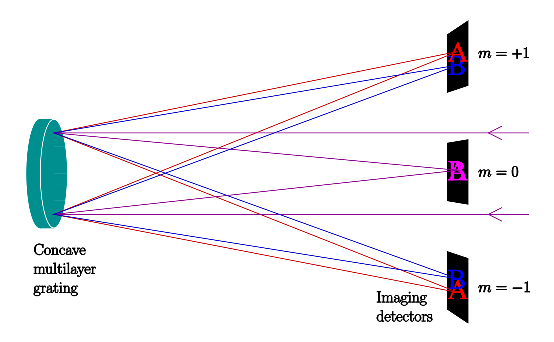
\includegraphics[height=2in]{figures/concave}
						\caption{Sketch of the optical system of MOSES}
						\label{optics}
					\end{subfigure}	
					~
					\begin{subfigure}[t]{0.49\textwidth}
						\centering
						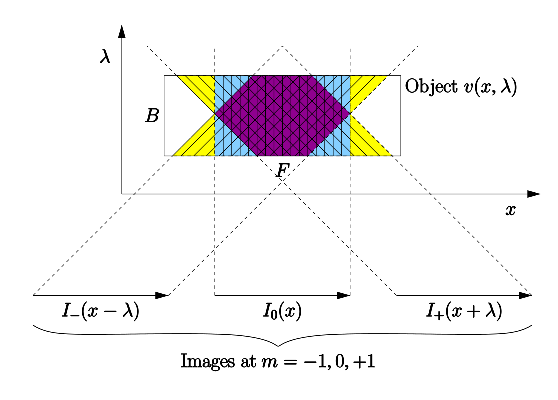
\includegraphics[height=2in]{figures/moses_cube}
						\caption{The analogue of Figure \ref{tomography} for the MOSES instrument.}
						\label{moses_tomo}
					\end{subfigure}	
					\caption{Two diagrams used to visualize the imaging system of the MOSES instrument. Figure \ref{optics} demonstrates how a bimodal spectral signal (a red `A' and a blue `B') are dispersed through the optical system. Figure \ref{moses_tomo} imagines the MOSES optical system as a 2D tomographic projection through a spatial-spectral cube. Figures courtesy of \cite{fox1}}
				\end{figure}
				MOSES is a CTIS that uses a single concave diffraction grating to produce images in three spectral orders, $m=-1,0,1$, as in Figure \ref{optics} (\cite{kankel1}).
				Since the diffraction grating of MOSES has rulings along only one direction, the dispersion is only in one direction. In the parlance of Figure \ref{tomography}, $\phi$ is restricted to the values of 0 and $\pi$ and then, without loss of generality, we can represent the 3D projections of Figure \ref{tomography} as 2D projections through a plane, as in Figure \ref{moses_tomo}.
				
				MOSES presents several challenges against achieving an accurate inversion. The most prevalent of these is the large, unknown point-spread function (PSF) of the instrument. The scale of this PSF is a compromise that allows MOSES to form images in three diffraction orders from a single optic (\cite{kankel1}).

			\subsubsection{ESIS}
			
				The EUV Snapshot Imaging Spectrograph (ESIS) is the next generation of a CTIS developed by Kankelborg and his research group. This instrument will be equipped with one large focusing primary mirror, and small, dedicated diffraction gratings for each detector. The first flight is planned for 2019 and the instrument will be equipped with four detectors to image the $m=1$ order in four separate dispersion directions. After the first flight has been completed, the system will undergo upgrades to install two additional gratings and detectors for a total of six tomographic projections. 
				\begin{figure}[h!]
					\centering
					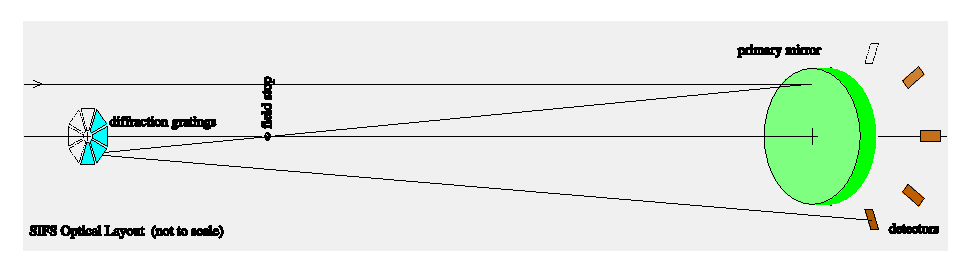
\includegraphics[width=0.8\textwidth]{figures/esis}
					\caption{A sketch following a single ray through the ESIS optical system. Image courtesy of Charles Kankelborg???}
					\label{esis_sketch}
				\end{figure}
				
				The tomographic projections of the ESIS instrument can be visualized in terms of Figure 1. The dedicated diffraction gratings are arranged in an octagonal pattern, producing projections at $\phi = 0, \; \pi/8, \; \pi/4, \; 3 \pi / 8, \; \pi /2, \; 5 \pi /8$ and $3 \pi /4$. Since these projections are not all in the same plane (unlike the MOSES arrangement), the inversion problem cannot be reduced to two dimensions and must be solved in 3D.
			
		\subsection{Previous Work}
			\label{pwork}
			
			The task of inverting MOSES data has already been undertaken by several research projects (\cite{inversion}, \cite{fox1}). The most effective inversion algorithm developed by these efforts is known as the \textit{smooth multiplicative algebraic reconstruction technique} (SMART) developed by \cite{kankel2} based off of earlier algebraic reconstruction techniques invented by \cite{Gordon70} and refined by \cite{Okamoto:91}. As discussed in Section \ref{inv_sec}, any CTIS inversion algorithm must use physical constraints to make the problem tractable. In the case of SMART, it uses the property that its solutions to the inversion problem must satisfy positivity, since intensity is a positive quantity (\cite{kankel2}).
			
			The result is a very efficient algorithm that has been successfully used to determine doppler shifts and line profiles of explosive events in He \textsc{ii} (\cite{rust1}).
			Unfortunately, it has proven difficult to convince SMART to produce physical inversions across the entire MOSES dataset. This unphysicality is mainly produced by an artifacts known colloquially as \textit{plaid}. As an example, in Figure \ref{plaid} we can see that the bright object in the center has been blurred at the angles: $\theta=-\pi/4, \; 0,$ and $\pi/4$ (with respect to the vertical) resulting in plaid. Such structures are considered to be unphysical since intensity is usually concentrated along horizontal spectral lines and not at angles of $\pi/4$.
			\begin{figure}[h!]
				\centering
				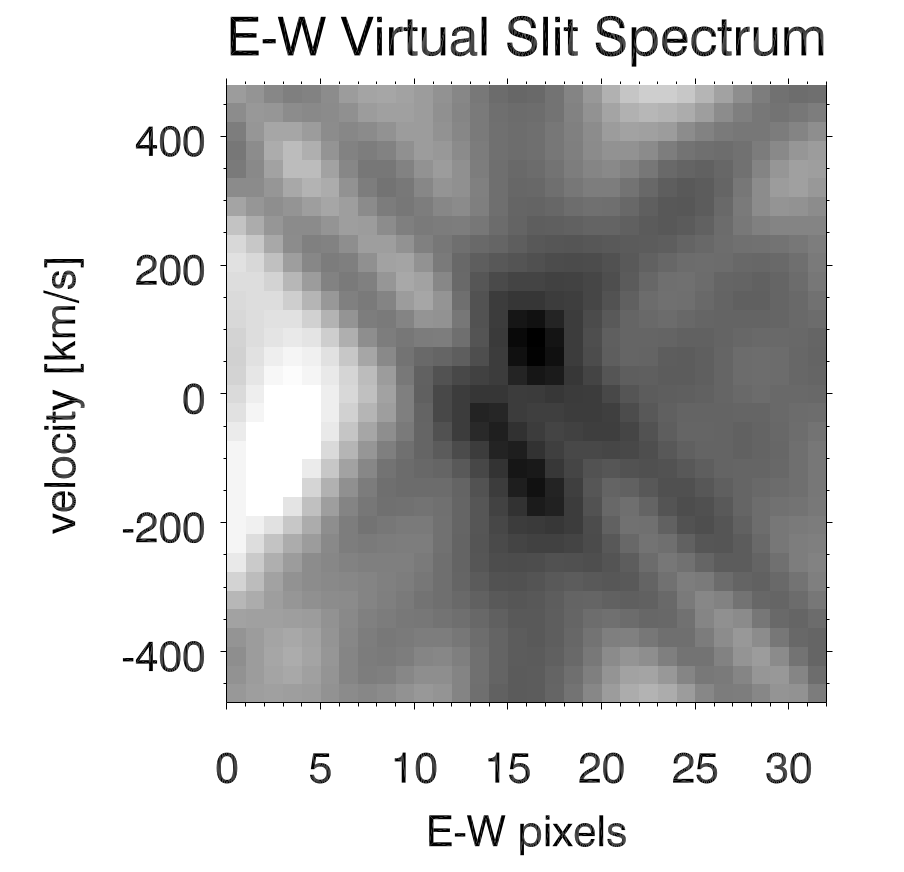
\includegraphics[width=0.3\textwidth]{figures/plaid}
				\caption{An example of plaid produced by SMART. The vertical dimension is the spectral dimension in units of relative doppler shift from line center, and the horizontal axis is position measured in pixels. Image courtesy of Thomas Rust.}
				\label{plaid}
			\end{figure}
			
			Plaid occurs whenever SMART attempts to invert a set of CTIS images with a background signal. Therefore, to yield plausible results using SMART, the background must be manually subtracted to isolate and successfully invert the area of interest. This operation prevents the creation of an automated, global inversion process for MOSES data.

		\subsection{Project Goals}
		
			Using the performance of SMART as a baseline, I would like to develop a more robust inversion algorithm to perform inversions of data produced by a CTIS such as MOSES and ESIS. The specific goals of my algorithm are to produce inversions with minimal to no plaid artifacts while maintaining a similar runtime to that of SMART. I will then use this algorithm to complete my ultimate goal of computing an inversion over the entire MOSES dataset, and later on ESIS after the instrument has been completed and launched.
		
	\section{Proposed Solution}
		\label{prop_sol}
			
		So far, all CTIS inversion algorithms have utilized physical constraints derived from first principles (such as positivity). This is not the only way however, instead an inversion algorithm could build physicality constraints based off of direct observation of the solar spectrum. For example, IRIS has been measuring the spectrum of the sun since 2013 (\cite{De Pontieu2014}), and has amassed a large dataset containing observations of the solar spectrum. An inversion algorithm that incorporates these observations has the potential to calculate inversions with greater accuracy because it would have the capability to eliminate solutions to the inversion problem that are inconsistent with the observations provided by IRIS.
			
		
		
		\subsection{Introduction to Neural Networks}
		
			Artificial neural networks are a tool used for non-linear
		
		\subsection{Inversion Using Neural Networks}
		\subsection{Preliminary Results}
	\section{Relevance to Heliophysics}
	\section{Project Timeline}
	

	\printbibliography

	
\end{document}

